% LLNCS manuscript for the CVPR 2026 Pan-cancer Segmentation challenge.
\documentclass[runningheads]{llncs}

\usepackage[T1]{fontenc}
\usepackage{amsmath}
\usepackage{graphicx}
\usepackage{array}
\usepackage[pagebackref=true,breaklinks=true,colorlinks,bookmarks=false]{hyperref}

\begin{document}

\title{RECIST-Anchored Lightweight 3D Lesion Segmentation for CPU-only Inference}
\titlerunning{RECIST-Anchored Lightweight 3D Lesion Segmentation}

\author{Zhou Jiang\inst{1}\orcidID{0000-0001-8146-2028} \and
Lisheng Wang\inst{1}\orcidID{0000-0003-3234-7511}}
\authorrunning{Z. Jiang and L. Wang}
\institute{School of Automation and Intelligent Sensing, Shanghai Jiao Tong University, Shanghai 200240, China\\
Corresponding author: Lisheng Wang, \email{lswang@sjtu.edu.cn}}

\maketitle

\begin{abstract}
RECIST-to-3D lesion segmentation aims to generate a volumetric lesion mask from a CT volume and a sparse 2D RECIST diameter marker. In Subtask 2 of the Pan-cancer Segmentation challenge, this task must be performed under strict CPU-only inference constraints, requiring both accurate prompt utilization and efficient implementation. Based on the public Lite ENSAM implementation and checkpoint, we fine-tune the lightweight model on the released training data and select the best validation checkpoint. We further introduce a RECIST-anchored inference strategy that treats the diameter marker as a lesion-specific geometric prior. Multi-label RECIST annotations are parsed into per-lesion prompts, localized prediction is performed around the marker, and RECIST-aware post-processing is applied to refine the final mask. The post-processing step merges the RECIST marker and its 3D radius-1 neighborhood as foreground seeds, retains connected components intersecting the corresponding marker, and performs hole filling within a local bounding box to avoid expensive full-volume operations. On 49 public validation cases, the proposed method achieved 0.7615 DSC and 0.8326 NSD, outperforming our same-machine rerun of the public Lite ENSAM checkpoint by 0.0623 DSC and 0.0855 NSD. The mean CPU inference time was 3.29 s per case, with no case exceeding the 60 s failure threshold. These results show that RECIST-anchored geometric constraints can improve prompt-to-3D lesion segmentation while maintaining efficient CPU-only deployment. Code is available at \url{https://github.com/zhoujiang18/recist-anchor}.

\keywords{RECIST-guided segmentation \and 3D lesion segmentation \and Pan-cancer CT segmentation \and Lightweight medical image segmentation \and Localized post-processing \and CPU-only inference}
\end{abstract}

\section{Introduction}
\label{sec:intro}

\subsection{Background and challenge}
Accurate lesion segmentation in volumetric CT images is important for tumor burden assessment, treatment planning, and longitudinal response evaluation. In routine clinical oncology, however, lesion size is often summarized using RECIST measurements~\cite{RECIST11}, where a radiologist annotates a 2D diameter on the axial slice that best represents the lesion. Such measurements are easy to acquire and remain widely used, but they are only a sparse description of a 3D object. Large-scale lesion resources such as DeepLesion have also shown that clinically recorded lesion diameters are valuable weak spatial annotations for learning lesion localization~\cite{deeplesion}. Nevertheless, a diameter line cannot directly capture irregular boundaries, through-plane extent, partial-volume effects, or multiple nearby components.

Subtask 2 of the Pan-cancer Segmentation challenge focuses on this practical gap: given a 3D CT image and a 2D RECIST diameter marker, a method must produce a 3D lesion mask. The task differs from fully automatic whole-body tumor segmentation because the RECIST marker provides a strong spatial prompt. It also differs from interactive segmentation because the inference must run on a laptop-like CPU-only environment. The challenge therefore requires a careful balance between segmentation accuracy, prompt utilization, memory footprint, and runtime. A method that predicts good masks but uses slow full-volume operations may fail individual cases once the per-case runtime exceeds 60 s.

\subsection{Related work}
General medical image segmentation has been strongly influenced by U-Net-style encoder-decoder architectures~\cite{U-Net}, volumetric extensions such as 3D U-Net~\cite{ThreeDUNet}, Dice-based 3D networks such as V-Net~\cite{VNet}, and self-configuring pipelines such as nnU-Net~\cite{nnUNet}. In abdominal and pan-cancer CT segmentation, FLARE challenges have highlighted the importance of computational efficiency, pseudo labeling, and robust post-processing~\cite{MedIA-FLARE21,FLARE22,FLARE23}. Foundation and promptable segmentation models, from the original Segment Anything Model~\cite{SAM} to medical adaptations such as MedSAM and MedSAM2~\cite{MedSAM,MedSAM2}, further motivate the use of sparse prompts to localize targets.

For the present task, Lite ENSAM~\cite{bjornstad2025lite} provides a particularly relevant starting point because it is lightweight and already supports prompt-like bounding-box information derived from lesion annotations. It was designed for efficient cancer segmentation in 3D CT and reports strong performance under limited resources. Nevertheless, directly applying a public checkpoint is not sufficient for this task: the public validation data, the containerized evaluation protocol, multi-lesion RECIST labels, and strict CPU runtime constraint expose failure modes that require additional checkpoint selection, prompt-consistent post-processing, and efficient implementation.

\subsection{Motivation and contributions}
Our main motivation is to exploit the fact that the RECIST marker is not merely an auxiliary annotation; it is a reliable geometric anchor for the target lesion. A plausible 3D lesion mask should contain the marker, remain spatially close to it, and suppress components that are disconnected from the prompted lesion. These requirements suggest a different design principle from generic lesion segmentation: instead of treating post-processing as a class-agnostic clean-up step, the RECIST marker can be used as a lesion-specific geometric constraint.

Building on this principle, we adapt the public Lite ENSAM checkpoint through supervised fine-tuning and validation-based checkpoint selection, rather than using the released model unchanged. The methodological novelty lies in the RECIST-anchored inference formulation: multi-label diameter markers are parsed as lesion-specific prompts, predicted components are selected according to their spatial relationship with the corresponding RECIST marker, and the RECIST line together with its 3D radius-1 neighborhood is introduced as a foreground seed before hole filling. This design improves prompt-neighborhood recall while retaining the irregular shape predicted by the network. To make this geometry practical for large CT scans, the computationally critical connected-component and hole-filling operations are restricted to a local bounding box around the predicted lesion and RECIST marker. This local formulation preserves the segmentation mask, avoids unnecessary full-volume operations, and keeps inference within the CPU-only runtime constraint.

\section{Method}
\label{sec:method}

Fig.~\ref{fig:pipeline} summarizes the proposed CPU-only inference framework. The method follows a single-model design: one fine-tuned lightweight network generates lesion logits, and all subsequent operations are deterministic functions of the RECIST marker and the predicted mask. This separation keeps the learned component compact while allowing the sparse clinical measurement to guide the final 3D topology.

\begin{figure}[!htbp]
\centering
\includegraphics[width=\textwidth]{imgs/fig1_overall_framework.png}
\caption{Overall framework of the proposed RECIST-anchored CPU-only inference method. The input CT volume and RECIST marker are loaded from NPZ files. RECIST markers are converted into per-lesion diameter prompts and used to define a local ROI. A fine-tuned Lite ENSAM model predicts lesion logits, after which RECIST seed union, local connected-component filtering, and hole filling produce the final uint8 multi-label NIfTI mask.}
\label{fig:pipeline}
\end{figure}

\subsection{Pre-processing}
\label{sec:preprocessing}

The challenge organizers provide preprocessed NPZ files, so we avoid expensive image preprocessing during inference. Each input contains a CT volume in the key \texttt{imgs}, RECIST annotations in \texttt{recist}, and spatial metadata. The image intensities have already been mapped to the range $[0,255]$, and the array layout is $(Z,Y,X)$. During containerized inference, only keys required for prediction are loaded: image, RECIST marker, spacing, direction, origin, and optional prompt-related keys. The ground-truth mask key is deliberately ignored during inference.

RECIST markers may contain multiple lesion labels. We therefore parse nonzero RECIST voxels label by label. For each label, the marker voxels are obtained with \texttt{np.argwhere} and grouped by their RECIST label. The implementation uses the lexicographically first and last nonzero voxels of each straight single-slice marker as the two line extremes, and these endpoints are used as the geometric prompt for the model. If a case contains no RECIST marker, the method returns an empty mask. This also provides a simple false-positive control for healthy or no-prompt cases.

No additional resampling is performed in the submitted configuration. This choice avoids interpolation cost and potential shape mismatches. Surface-distance evaluation still uses the spacing stored in the NPZ file. The method therefore operates in the provided voxel grid and relies on RECIST-localized inference to limit the region of interest.

\subsection{Network and prompt-based prediction}
\label{sec:network}

The segmentation backbone is based on Lite ENSAM~\cite{bjornstad2025lite}, a compact 3D CT lesion segmentation model with a SegResNet-style encoder~\cite{Myronenko2018SegResNet} and prompt-conditioned decoder. In our submitted model, the instantiated network contains approximately 1.32 million trainable parameters. We keep the model lightweight because Subtask 2 evaluates inference on CPU without GPU acceleration.

The network receives a local CT crop and RECIST-derived prompts. The prompt is represented through diameter endpoints and propagated through the decoder as bounding-box-like spatial information. For network inference, the RECIST-derived prompt box is cropped with a 24-voxel margin in each dimension before downsampling and padding. This crop margin is used only to define the model input region and is distinct from the one-voxel local bounding-box expansion used later for post-processing. This is important because the task is prompt-to-mask rather than unconstrained whole-body segmentation. The model predicts a logit map for each lesion label in the crop. The crop is then mapped back to the original CT volume.

We considered adding the RECIST marker as an explicit second image channel. However, this would require modifying the first convolutional layer, adapting pretrained weights, retraining the image encoder, and revalidating the containerized inference path. Since the public Lite ENSAM architecture already uses RECIST-derived box prompts, we retained the original prompt path and focused on robust training selection and inference-time RECIST geometry.

\subsection{Training and checkpoint selection}
\label{sec:training}

We initialized from the public Lite ENSAM checkpoint and performed supervised fine-tuning on the provided training data. The training objective follows the public implementation and uses a Dice plus cross-entropy compound loss, implemented as DiceCE loss~\cite{LossOdyssey}. The optimizer is the AdamMuon variant used in the Lite ENSAM training code, with AdamW-style updates for non-matrix parameters~\cite{AdamW}. We searched over random seeds, learning rates, and epoch sizes. The best checkpoint was selected by validation DSC/NSD. The public validation set was therefore used as a development set for checkpoint and module selection; the reported validation results document development-stage performance before hidden-test evaluation.

The final selected checkpoint used seed 2032, learning rate $1\times 10^{-4}$, batch size 1, and 12,000 fine-tuning iterations. This was implemented as two fixed-length pseudo-epochs with 6000 iterations per epoch. Additional low-learning-rate fine-tuning from the selected checkpoint, decoder/prompt-only fine-tuning, boundary-loss fine-tuning, and intensity-augmentation fine-tuning were also tested, but none improved the final validation score. We therefore used the best validation checkpoint rather than the latest checkpoint.

Unlabeled images and partially labeled data were not used in the final method. Pseudo labels generated by previous FLARE winning algorithms were not used. Algorithm distillation was not used. These choices simplify the proposed method and avoid introducing uncertain labels close to the submission deadline.

\subsection{RECIST-aware post-processing}
\label{sec:postprocessing}

The final post-processing is designed around the RECIST marker rather than around global foreground probability alone. For each nonzero RECIST label, the corresponding predicted mask is processed independently. The RECIST marker itself and its 3D radius-1 neighborhood are first merged into the predicted binary mask for that label. This \emph{RECIST seed-union} rule encodes the assumption that the annotated diameter should lie inside the target lesion, improves recall around the most reliable foreground evidence, and does not require ground truth or an additional model.

The procedure can be written compactly as follows. Let $P_l \subset \Omega$ denote the predicted foreground voxels for lesion label $l$, and let $R_l \subset \Omega$ denote the corresponding RECIST marker in the image domain $\Omega$. We construct a RECIST-augmented seed mask and a local processing domain as
\begin{align}
S_l &= P_l \cup \delta_1(R_l), \label{eq:seed_union}\\
\Omega_l &= \operatorname{bbox}\left(S_l \cup R_l\right) \oplus 1, \label{eq:local_box}
\end{align}
where $\delta_1(\cdot)$ is a 3D binary dilation with a radius of one voxel, $\operatorname{bbox}(\cdot)$ denotes the tight bounding box, and $\oplus 1$ expands it by one voxel in each direction.

Connected components are then computed on the union mask, following the classical connected-component labeling principle in digital picture processing~\cite{RosenfeldPfaltz1966}. Components that intersect the corresponding RECIST marker are retained, while components disconnected from the marker are discarded as likely false positives. If no component intersects the marker, the largest component is retained as a conservative fallback. Binary hole filling is subsequently applied to the retained local mask to remove small internal gaps. The result is written back using the original lesion label, so multi-lesion cases keep labels such as 1, 2, 3, and 4 instead of being collapsed into a binary mask.

Formally, if $\{C_{l,k}\}_{k=1}^{N_l}$ are the connected components of $S_l$ within $\Omega_l$, the retained component index set and final mask are
\begin{align}
\mathcal{I}_l &=
\begin{cases}
\{k \mid C_{l,k}\cap R_l \neq \emptyset\}, & \text{if such components exist},\\
\{\arg\max_k |C_{l,k}|\}, & \text{otherwise},
\end{cases}
\label{eq:component_selection}\\
\hat{Y}_l &= \operatorname{Fill}\left(\bigcup_{k\in\mathcal{I}_l} C_{l,k}\right).
\label{eq:final_mask}
\end{align}
where $\operatorname{Fill}(\cdot)$ denotes binary hole filling. The complete multi-label output is obtained by assigning label $l$ to voxels in $\hat{Y}_l$ for each RECIST label. Labels are processed in ascending numerical order; if masks from different RECIST labels overlap after post-processing, the later label overwrites the earlier one, which provides a deterministic conflict-resolution rule matching the implementation.

A direct full-volume implementation of this RECIST-aware post-processing can be slow for thick CT scans. For example, a validation case of shape $(554,512,512)$ caused a severe runtime bottleneck when connected-component analysis was applied to the full volume. For local post-processing, we compute the tight bounding box of the union between the seeded prediction and RECIST marker, expand it by one voxel as in Eq.~\eqref{eq:local_box}, and restrict connected-component analysis and hole filling to that local box. This one-voxel expansion is separate from the 24-voxel margin used for network-input cropping. The local-bounding-box implementation produced zero voxel differences compared with the full-volume version while reducing the runtime of the largest case from hundreds of seconds on a slower CPU to approximately 10 s. The acceleration is therefore algorithmically lossless for the tested validation cases.

Operationally, the localized post-processing has five deterministic steps. First, the raw multi-label prediction is split according to the nonzero RECIST labels. Second, for each lesion label, the RECIST diameter voxels and their 3D radius-1 neighborhood are inserted as foreground seeds. Third, a local bounding box is computed from the union of the seeded prediction and the RECIST marker, so all expensive connected-component operations are restricted to a small ROI. Fourth, only connected components that intersect the corresponding RECIST marker are retained; disconnected components are removed as remote false positives. Fifth, hole filling is applied inside the local ROI, and the retained mask is written back to the full image with its original lesion label.

\section{Experiments}
\label{sec:experiments}

\subsection{Dataset and evaluation measures}
\label{sec:dataset}

The challenge organizers curate CT scans from multiple public and licensed sources and release them in a unified NPZ format for Subtask 2. Each case provides a 3D CT image, a 2D RECIST diameter marker, and spatial metadata as input, and the expected output is a 3D lesion segmentation mask. In this work, we use only the official files released for Subtask 2 and do not introduce additional private data.

We evaluated on the 49 public validation NPZ cases available locally. The two accuracy metrics are Dice Similarity Coefficient (DSC)~\cite{Dice1945} and Normalized Surface Dice (NSD), a spacing-aware surface-overlap metric related to the surface Dice formulation used for clinically oriented segmentation assessment~\cite{SurfaceDice}. DSC measures volumetric overlap:
\begin{equation}
\mathrm{DSC}(G,S)=\frac{2|G\cap S|}{|G|+|S|},
\end{equation}
where $G$ is the ground truth and $S$ is the predicted segmentation. NSD measures the fraction of surface elements that are within a tolerance distance from the opposite surface. We used the challenge-style spacing-aware NSD implementation with a 2 mm tolerance. For multi-lesion cases, metrics were computed per nonzero ground-truth label and averaged.

Efficiency is also part of the challenge ranking, consistent with the broader view that biomedical challenge rankings should consider multiple task-relevant metrics rather than a single accuracy number~\cite{ChallengeR}. The Task 2 Docker is evaluated without GPU and with an 8 GB memory limit. A case exceeding 60 s is considered failed. Running times below 45 s are within the official tolerance.

\subsection{Implementation details}
\label{sec:implementation}

Table~\ref{table:env} summarizes the development environment used for local experiments. Training and checkpoint search were performed on GPUs, while all validation results for the submitted method used CPU-only inference. The container entry point explicitly sets \texttt{CUDA\_VISIBLE\_DEVICES=""}.

\begin{table}[!htbp]
\caption{Development environment and final inference setting.}
\label{table:env}
\centering
\begin{tabular}{ll}
\hline
Operating system & Ubuntu Linux, kernel 5.4 \\
\hline
CPU for local validation & Intel Core i9-10920X, 12 cores / 24 threads \\
\hline
RAM & 128 GB local memory; container tested with 8 GB limit \\
\hline
GPU for training/search & 2 NVIDIA GeForce RTX 3090 GPUs, 24 GB each \\
\hline
Inference GPU & None for submitted inference \\
\hline
Programming language & Python 3.8 \\
\hline
Framework and libraries & PyTorch 1.12, NumPy 1.23, SciPy 1.8, NiBabel 5.1 \\
\hline
Output format & uint8 NIfTI files with multi-label lesion masks \\
\hline
\end{tabular}
\end{table}

Table~\ref{table:training} lists the main training protocol for the selected checkpoint. We report only settings used by the final selected training run. Other exploratory runs are discussed in Sec.~\ref{sec:ablation}.

\begin{table}[!htbp]
\caption{Training protocol for the selected checkpoint.}
\label{table:training}
\centering
\begin{tabular}{ll}
\hline
Network initialization & Public Lite ENSAM checkpoint \\
\hline
Training strategy & Supervised fine-tuning / checkpoint selection \\
\hline
Batch size & 1 \\
\hline
Total epochs & 2 fixed-length pseudo-epochs \\
\hline
Total fine-tuning iterations & 12,000 \\
\hline
Epoch size & 6000 iterations \\
\hline
Optimizer & AdamMuon / AdamW-style optimizer from Lite ENSAM code \\
\hline
Learning rate & $1\times 10^{-4}$ \\
\hline
Weight decay & $1\times 10^{-4}$ \\
\hline
Loss function & DiceCE loss \\
\hline
Model selection & Best validation Dice checkpoint \\
\hline
Number of parameters & 1.32M \\
\hline
Unlabeled data & Not used \\
\hline
Pseudo labels & Not used \\
\hline
\end{tabular}
\end{table}

\section{Results and Discussion}
\label{sec:results}

\subsection{Quantitative validation results}
\label{sec:quantitative}

Table~\ref{tab:final-results} compares the original Lite ENSAM reference, our same-machine rerun of the public Lite ENSAM checkpoint, and the main stages of the proposed method. The reported Lite ENSAM score is included only as an external reference from the public release, because differences in validation files, RECIST handling, runtime environment, and metric implementation may affect direct comparability. The same-machine rerun is used as the primary fair baseline, because it uses the same 49 public validation NPZ files, the same workstation, the provided \texttt{recist} marker key as input, the same container setting, and the same metric implementation as our submitted method.

The final method achieved 0.7615 DSC and 0.8326 NSD, compared with 0.6992 DSC and 0.7471 NSD for the same-machine Lite ENSAM rerun. This corresponds to absolute improvements of 0.0623 DSC and 0.0855 NSD, or relative improvements of 8.9\% and 11.4\%, respectively. The improvement over the fine-tuned model alone is also consistent: RECIST-aware post-processing increases DSC from 0.7424 to 0.7615 and NSD from 0.8005 to 0.8326, corresponding to relative gains of 2.6\% and 4.0\%. We therefore use the controlled same-machine rerun and the fine-tuned-only checkpoint as the main evidence for the proposed adaptation; the public Lite ENSAM report is retained in the table as contextual information rather than as the primary comparison protocol.

\begin{table}[!htbp]
\caption{Quantitative results on the public validation set. Metrics are averaged over 49 validation cases. The public Lite ENSAM report is included for external reference; the same-machine rerun is the primary controlled baseline.}
\label{tab:final-results}
\centering
\resizebox{\textwidth}{!}{%
\begin{tabular}{lcccc}
\hline
Method & Evaluation setting & DSC & NSD & Mean CPU time \\
\hline
Lite ENSAM public report~\cite{bjornstad2025lite} & Reported by authors & 0.7606 & 0.7899 & -- \\
Lite ENSAM public checkpoint & Same-machine rerun, actual RECIST & 0.6992 & 0.7471 & 4.03 s \\
Fine-tuned selected model only & Same-machine containerized evaluation & 0.7424 & 0.8005 & 3.98 s \\
RECIST CC + hole filling, network ROI margin 24 & Same-machine containerized evaluation & 0.7558 & 0.8185 & 8.83 s \\
Final method with local post-processing & Same-machine containerized evaluation & \textbf{0.7615} & \textbf{0.8326} & \textbf{3.29 s} \\
\hline
\end{tabular}
}
\end{table}

Fig.~\ref{fig:performance} visualizes the same comparison. The performance progression shows that the gain is not produced by a single implementation detail: supervised fine-tuning improves the baseline model, while RECIST-aware component selection and seed union further refine the spatial support of the lesion. The larger relative improvement in NSD than DSC suggests that the marker-anchored post-processing reduces boundary errors and disconnected false positives, both of which are strongly reflected by surface-based evaluation.

\begin{figure}[!htbp]
\centering
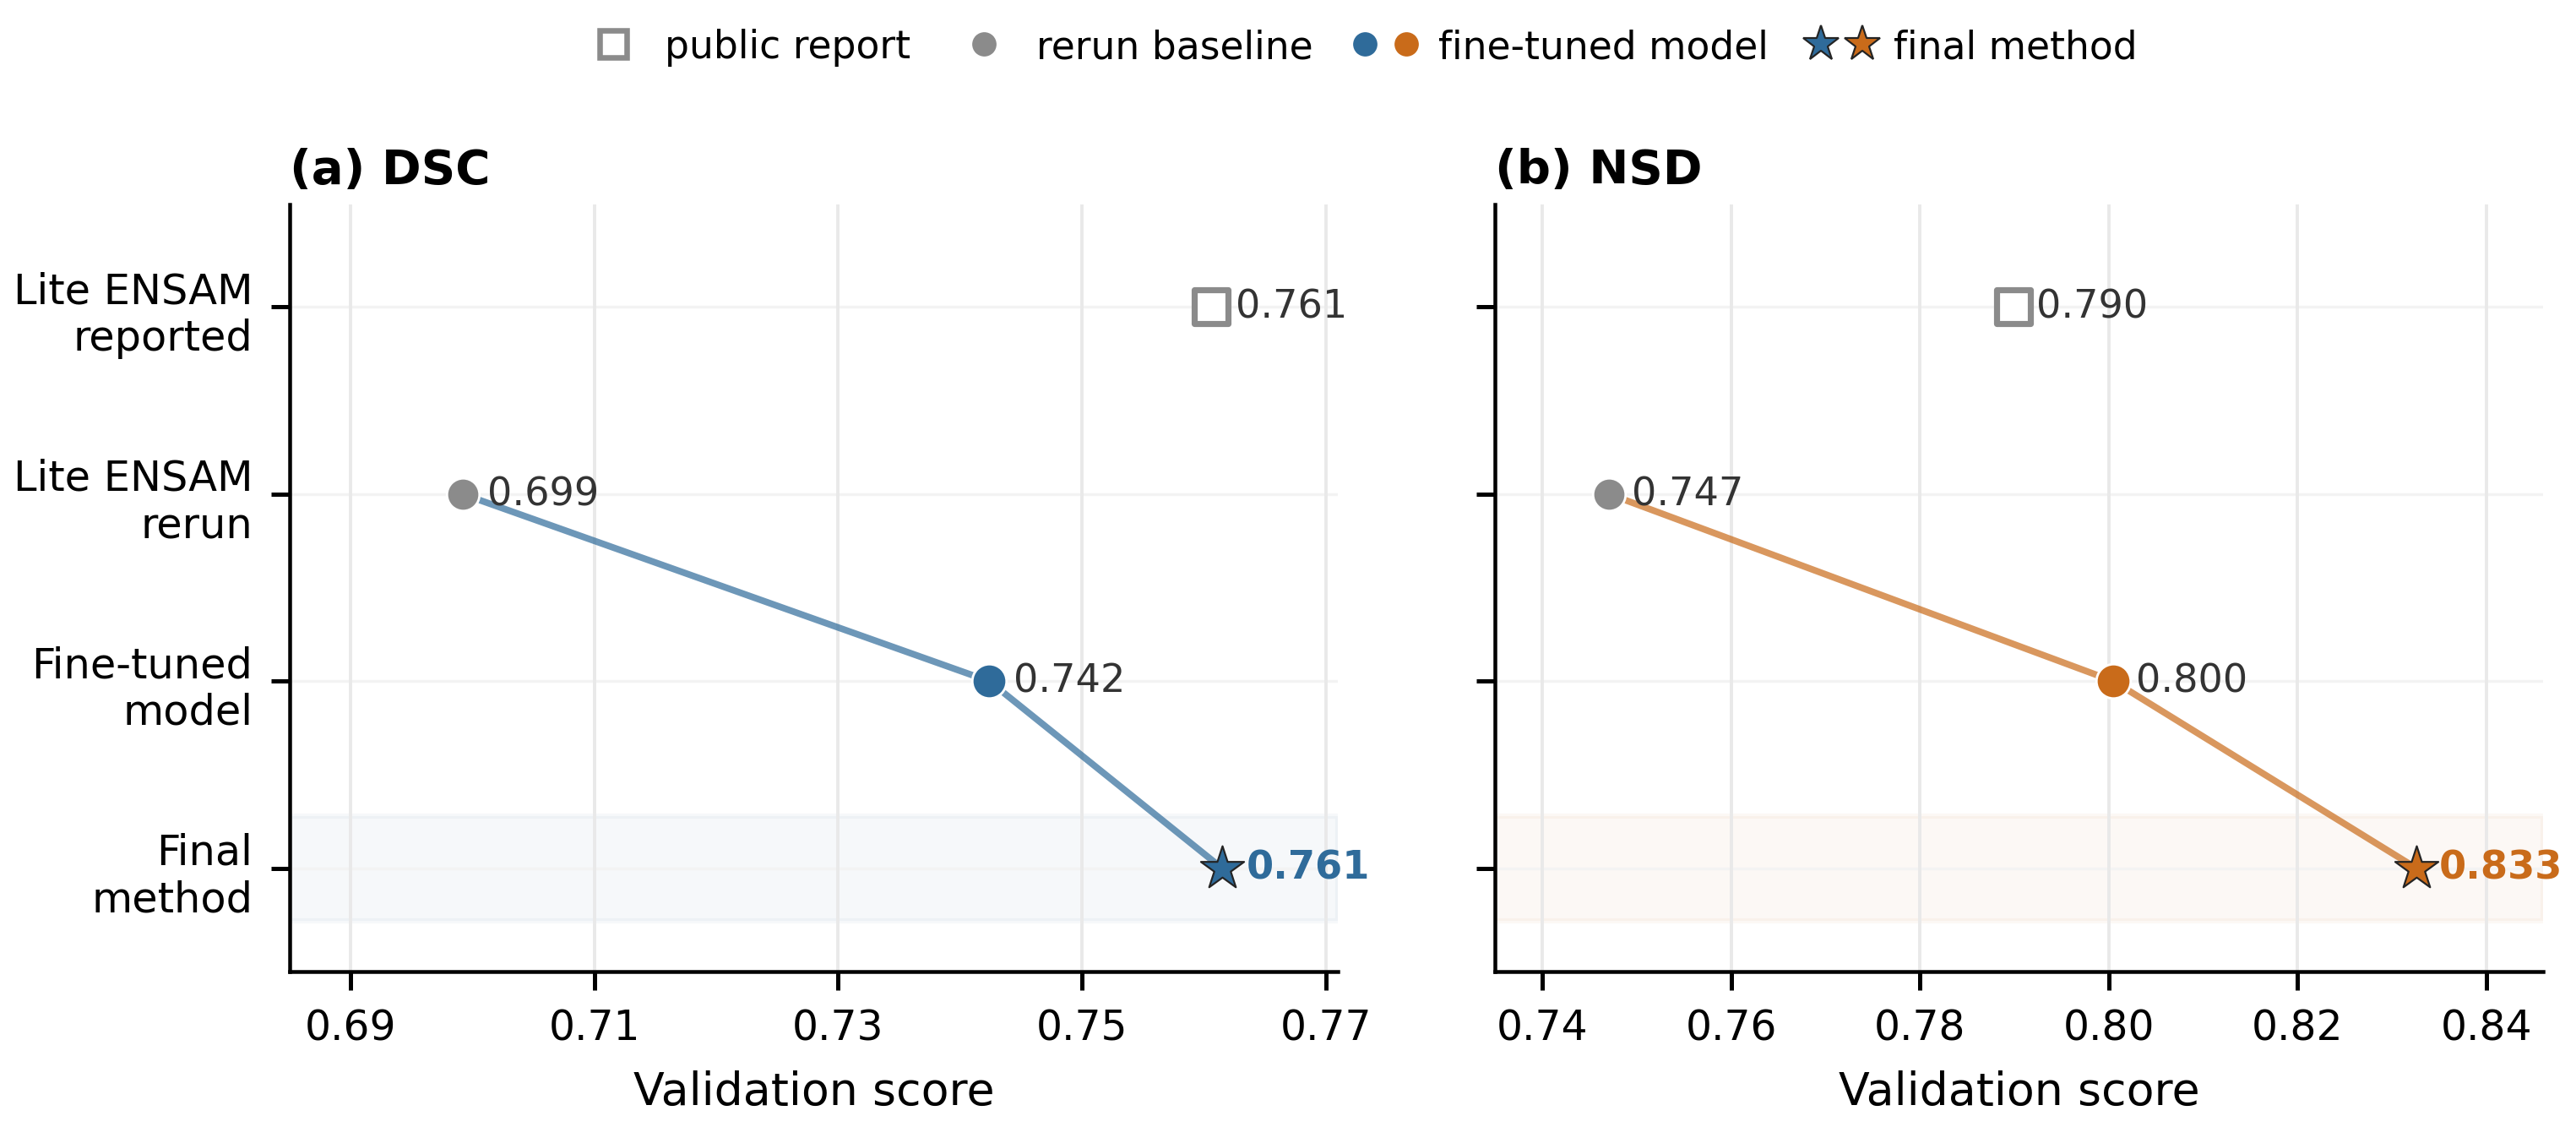
\includegraphics[width=0.85\textwidth]{imgs/medai_performance_progression.png}
\caption{Performance progression on the public validation set. Hollow squares denote the public Lite ENSAM report, gray circles denote the rerun baseline, colored circles denote the fine-tuned model, and stars denote the final method. The proposed method improves both DSC and NSD compared with the rerun baseline and the fine-tuned checkpoint alone.}
\label{fig:performance}
\end{figure}

\subsection{Ablation study}
\label{sec:ablation}

Table~\ref{tab:ablation} summarizes the module-level ablation of the final method. Starting from the selected fine-tuned model output, RECIST-aware connected-component selection and hole filling improved DSC from 0.7424 to 0.7558 and NSD from 0.8005 to 0.8185, giving absolute gains of 0.0134 DSC and 0.0180 NSD. Adding the 3D radius-1 RECIST seed union further improved DSC to 0.7615 and NSD to 0.8326, showing that explicitly enforcing the RECIST neighborhood as foreground recovers useful lesion voxels near the prompt. The final local-bounding-box implementation did not change the output masks; it produced zero voxel differences compared with the full-volume version. However, it reduced mean CPU time from 8.94 s to 3.29 s, a 63.2\% reduction, and reduced the maximum official-like runtime from 27.17 s to 8.86 s, a 67.4\% reduction.

\begin{table}[!htbp]
\caption{Module-level ablation on the public validation set. Metrics are averaged over 49 validation cases.}
\label{tab:ablation}
\centering
\resizebox{\textwidth}{!}{%
\begin{tabular}{lcccc}
\hline
Configuration & DSC & NSD & Mean CPU time & Main effect \\
\hline
Fine-tuned selected model only & 0.7424 & 0.8005 & 3.98 s & Network prediction baseline \\
+ RECIST CC + hole filling, network ROI margin 24 & 0.7558 & 0.8185 & 8.83 s & Suppress remote false positives \\
+ 3D radius-1 RECIST seed union & \textbf{0.7615} & \textbf{0.8326} & 8.94 s & Improve prompt-neighborhood recall \\
+ Local-bounding-box post-processing & \textbf{0.7615} & \textbf{0.8326} & \textbf{3.29 s} & Preserve masks while accelerating CPU inference \\
\hline
\end{tabular}
}
\end{table}

Fig.~\ref{fig:module-ablation} shows the same module ablation visually. The accuracy gain comes mainly from RECIST-anchored component selection and seed union, whereas the local-bounding-box implementation is a mask-preserving efficiency improvement. This separation is useful for interpreting the method: the RECIST geometry improves segmentation quality, while the localized implementation makes the same geometry feasible under strict CPU inference constraints.

\begin{figure}[!htbp]
\centering
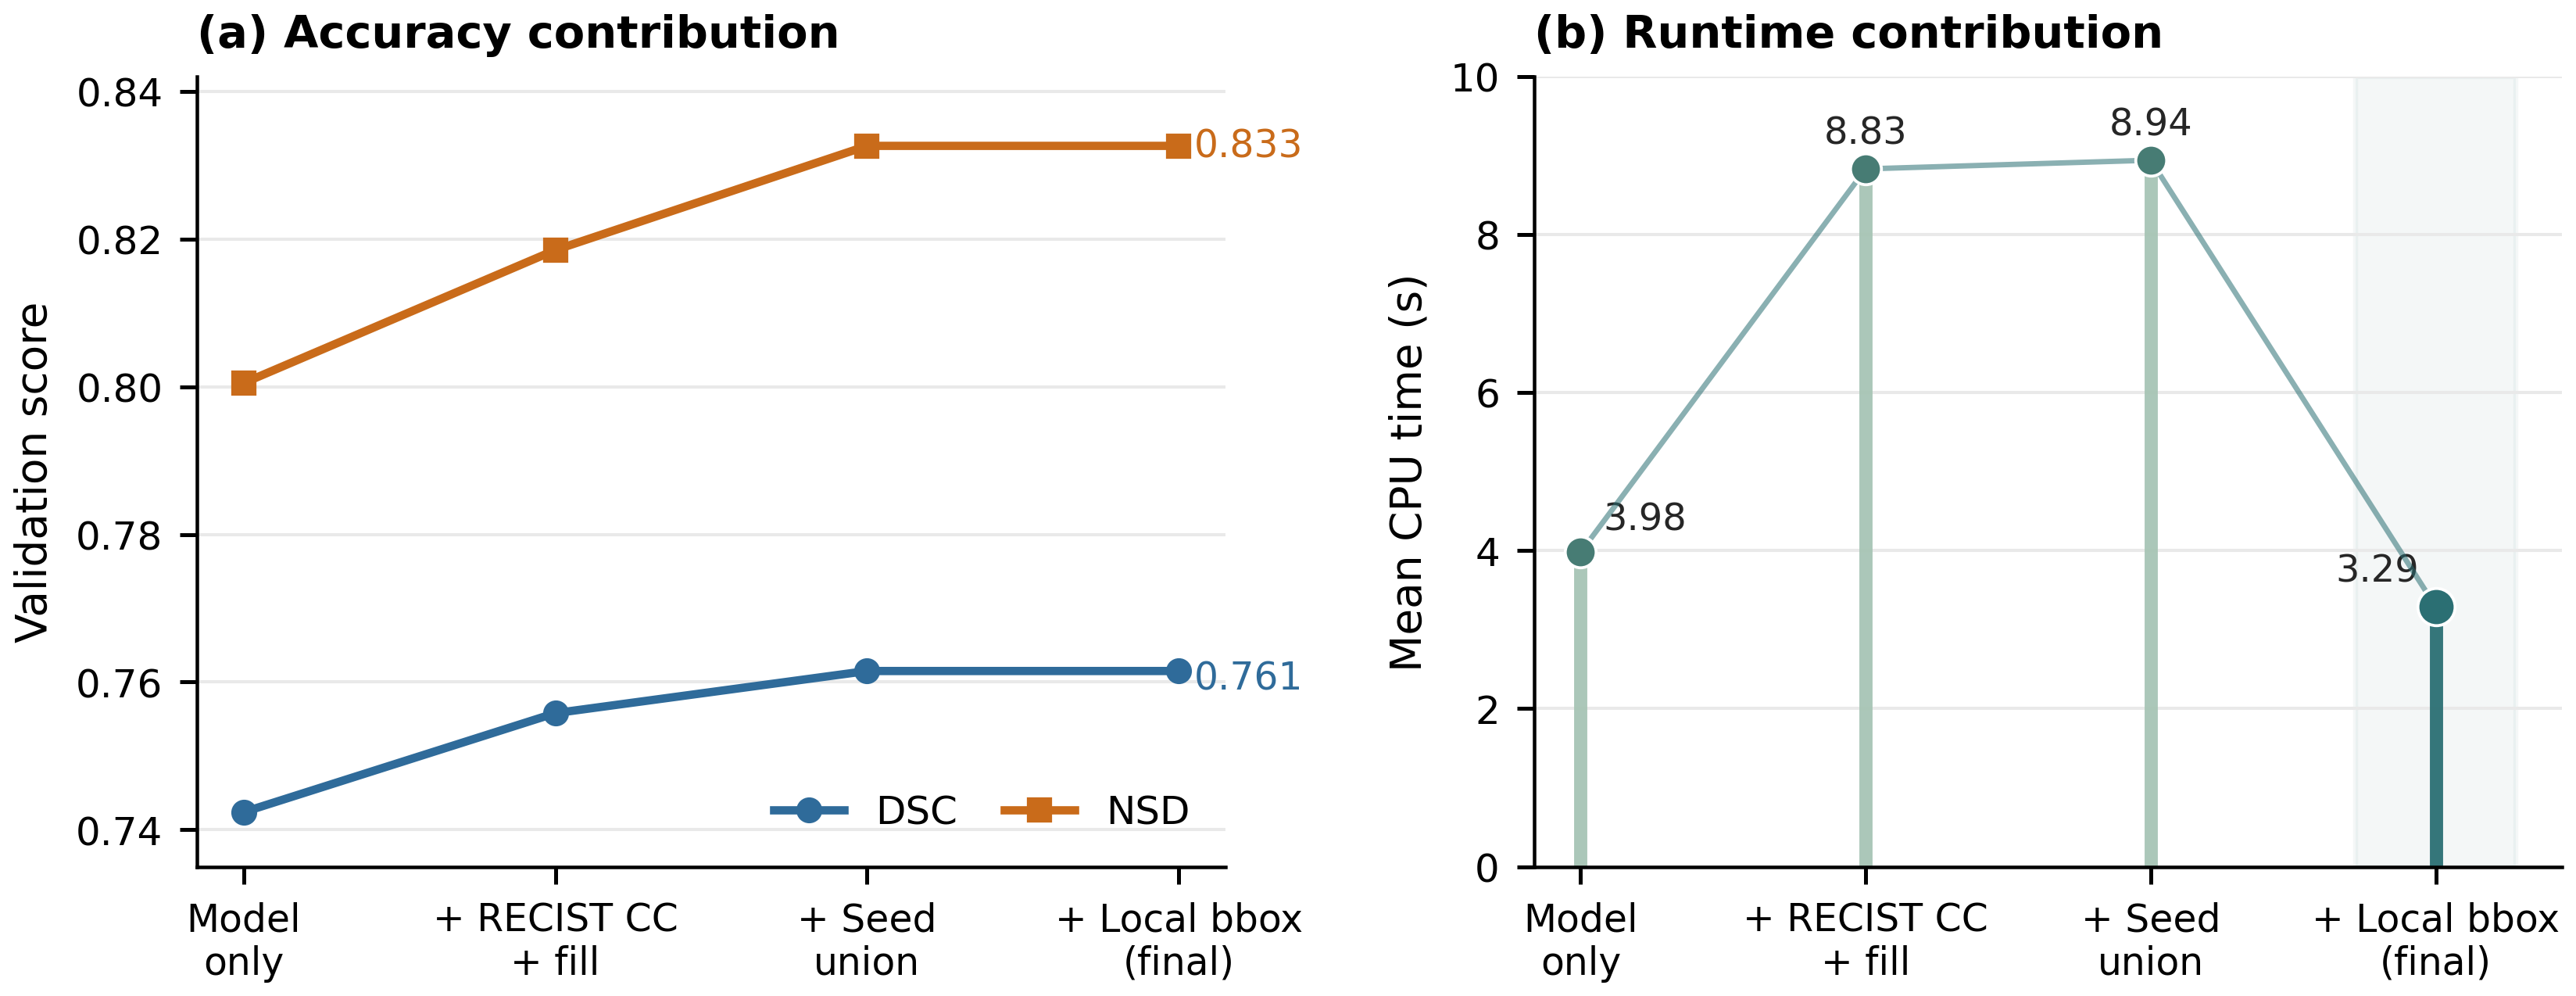
\includegraphics[width=0.9\textwidth]{imgs/medai_module_ablation.png}
\caption{Module ablation on the public validation set. Panel (a) shows the DSC/NSD contribution of each module, and panel (b) shows the corresponding mean CPU runtime. RECIST-aware post-processing improves segmentation accuracy, while local-bounding-box post-processing preserves the final mask and substantially reduces CPU runtime.}
\label{fig:module-ablation}
\end{figure}

We also tested several variants that were not retained. A 3$\times$ test-time augmentation run obtained 0.7417 DSC and 0.7974 NSD, a two-model ensemble obtained 0.7383 DSC and 0.7953 NSD, and a weighted ensemble with RECIST filling obtained 0.7469 DSC and 0.8089 NSD. These results suggest that simply averaging predictions does not address the dominant error mode in this task, which is spatial inconsistency with the RECIST marker. Boundary-loss fine-tuning reached 0.7352 DSC and 0.8000 NSD, while decoder/prompt-only low-learning-rate fine-tuning reached 0.7233 DSC and 0.7880 NSD. Ellipsoid constraints derived from the RECIST diameter, volume guards, slice-wise propagation, adaptive crop margins, and morphological smoothing also did not consistently improve both DSC and NSD. In practice, hard geometric priors can over-constrain irregular lesions. The softer strategy of retaining components anchored at the RECIST marker while preserving the network-predicted shape was more robust.

\subsection{Qualitative validation results}
\label{sec:qualitative}

Fig.~\ref{fig:qualitative} shows two high-scoring cases and two difficult cases. Cases 0097 and 0027 illustrate compact lesions whose RECIST marker lies near the central slice and whose through-plane extent is well captured by the ROI crop. Cases 0069 and 0048 illustrate more difficult situations with elongated structures, nearby high-contrast anatomy, and boundary disagreement between prediction and ground truth. Even in these difficult cases, the RECIST marker helps keep the prediction spatially aligned with the target lesion and suppresses remote false positives.

\begin{figure}[!htbp]
\centering
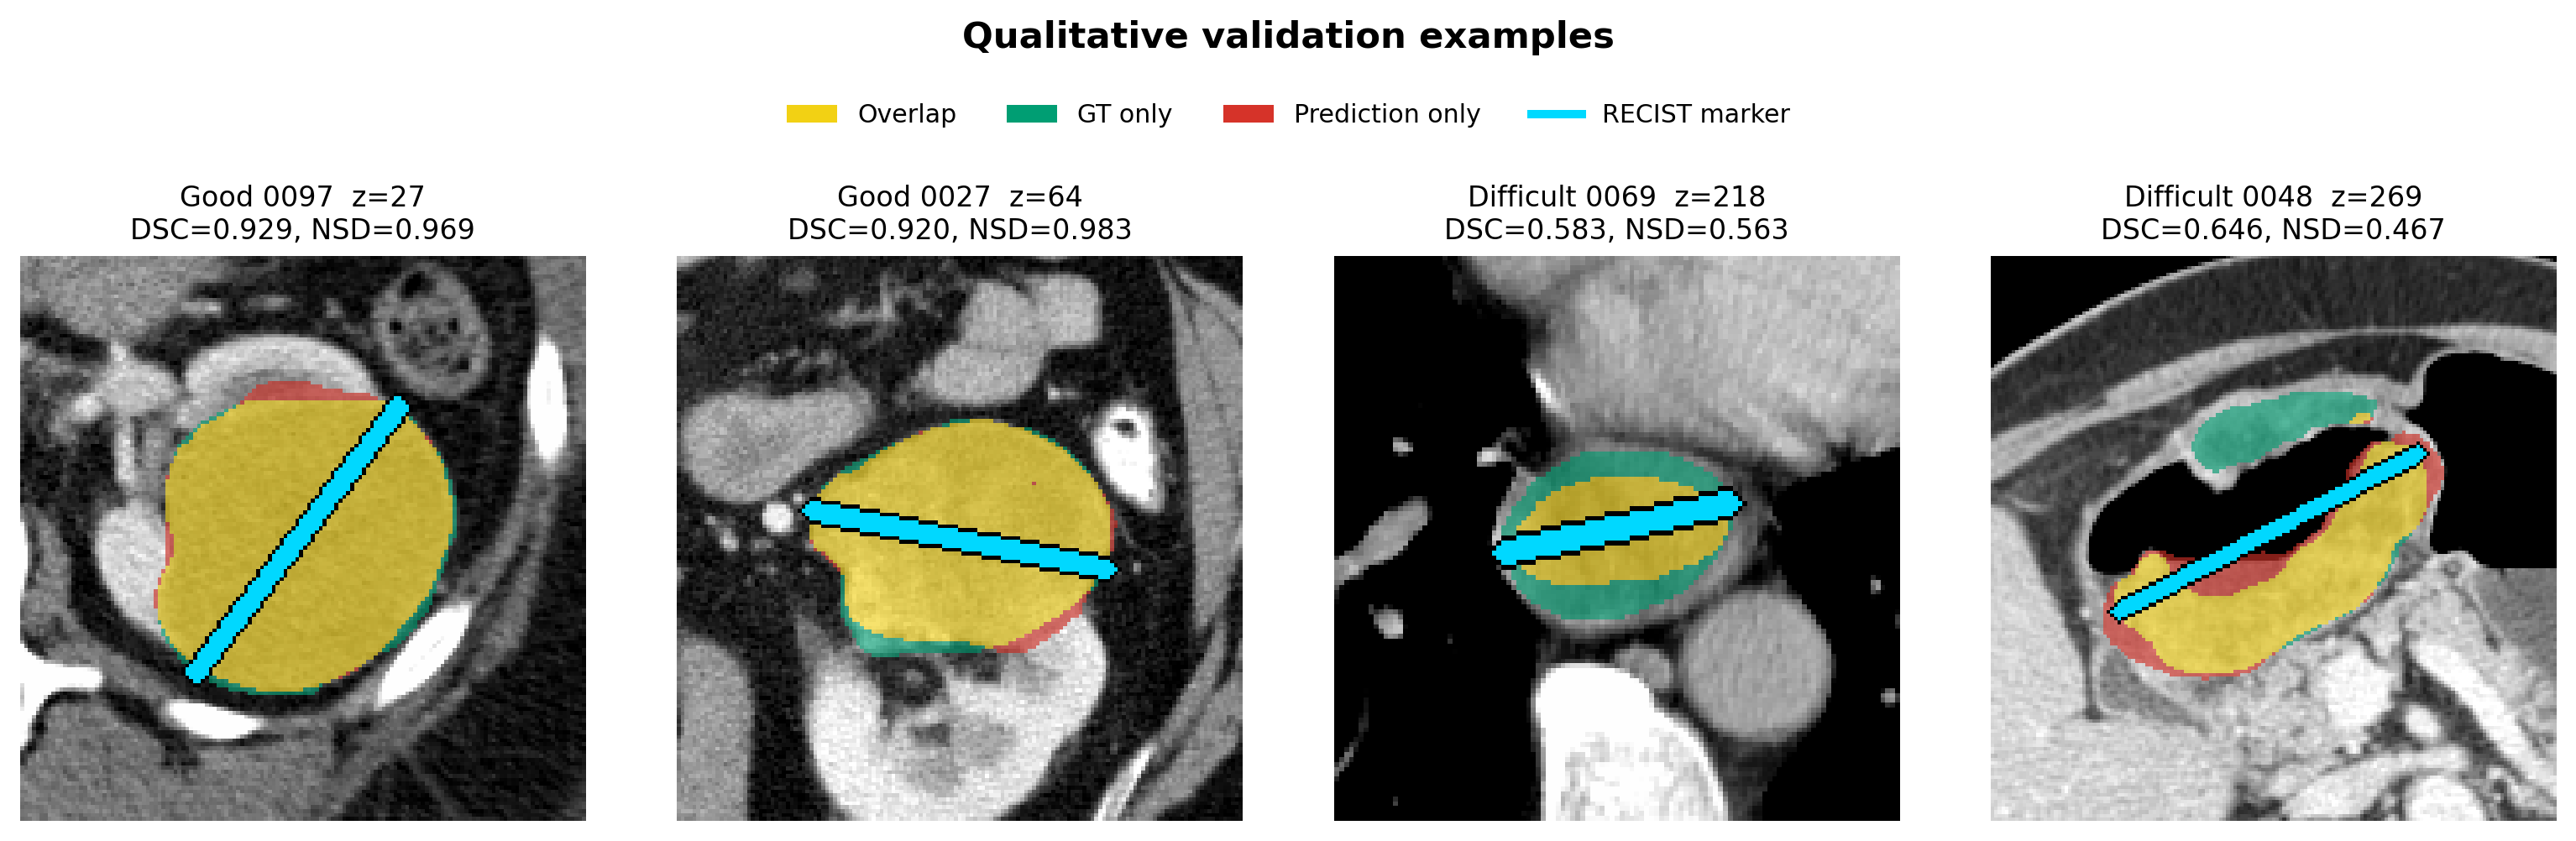
\includegraphics[width=\textwidth]{imgs/medai_qualitative_examples.png}
\caption{Qualitative examples on public validation cases. Yellow denotes overlap between prediction and ground truth, green denotes ground truth only, red denotes prediction only, and cyan denotes the RECIST marker, drawn with a black outline for visibility. The first two cases are high-scoring examples, while the last two illustrate typical difficult cases with boundary disagreement or partial under-segmentation.}
\label{fig:qualitative}
\end{figure}

\subsection{Segmentation efficiency}
\label{sec:efficiency}

Table~\ref{tab:efficiency} reports representative CPU-only runtimes for cases of different depths. Since Task 2 forbids GPU use during inference, GPU memory is zero by design. The final evaluation was performed with an 8 GB container memory limit. All representative cases are well below the 60 s failure threshold.

\begin{table}[!htbp]
\caption{Representative CPU-only efficiency results on public validation cases. Image size is reported as $(Z,Y,X)$.}
\label{tab:efficiency}
\centering
\begin{tabular}{lccc}
\hline
Case ID & Image size & Runtime (s) & GPU memory \\
\hline
0001 & $(55,512,512)$ & 0.76 & 0 MB \\
0051 & $(100,512,512)$ & 3.13 & 0 MB \\
0017 & $(151,512,512)$ & 3.84 & 0 MB \\
0019 & $(215,512,512)$ & 4.11 & 0 MB \\
0099 & $(334,512,512)$ & 7.26 & 0 MB \\
0063 & $(448,512,512)$ & 8.03 & 0 MB \\
0048 & $(499,512,512)$ & 8.11 & 0 MB \\
0029 & $(554,512,512)$ & 8.86 & 0 MB \\
\hline
\end{tabular}
\end{table}

Fig.~\ref{fig:runtime} shows the full 49-case runtime distribution from the validation sanity run. The maximum case runtime in the full sanity video was 9.87 s, and the maximum runtime in the official-like metric run was 8.86 s. The difference comes from repeated Docker runs and normal CPU variation. In both settings, every case remained far below 45 s and 60 s.

\begin{figure}[!htbp]
\centering
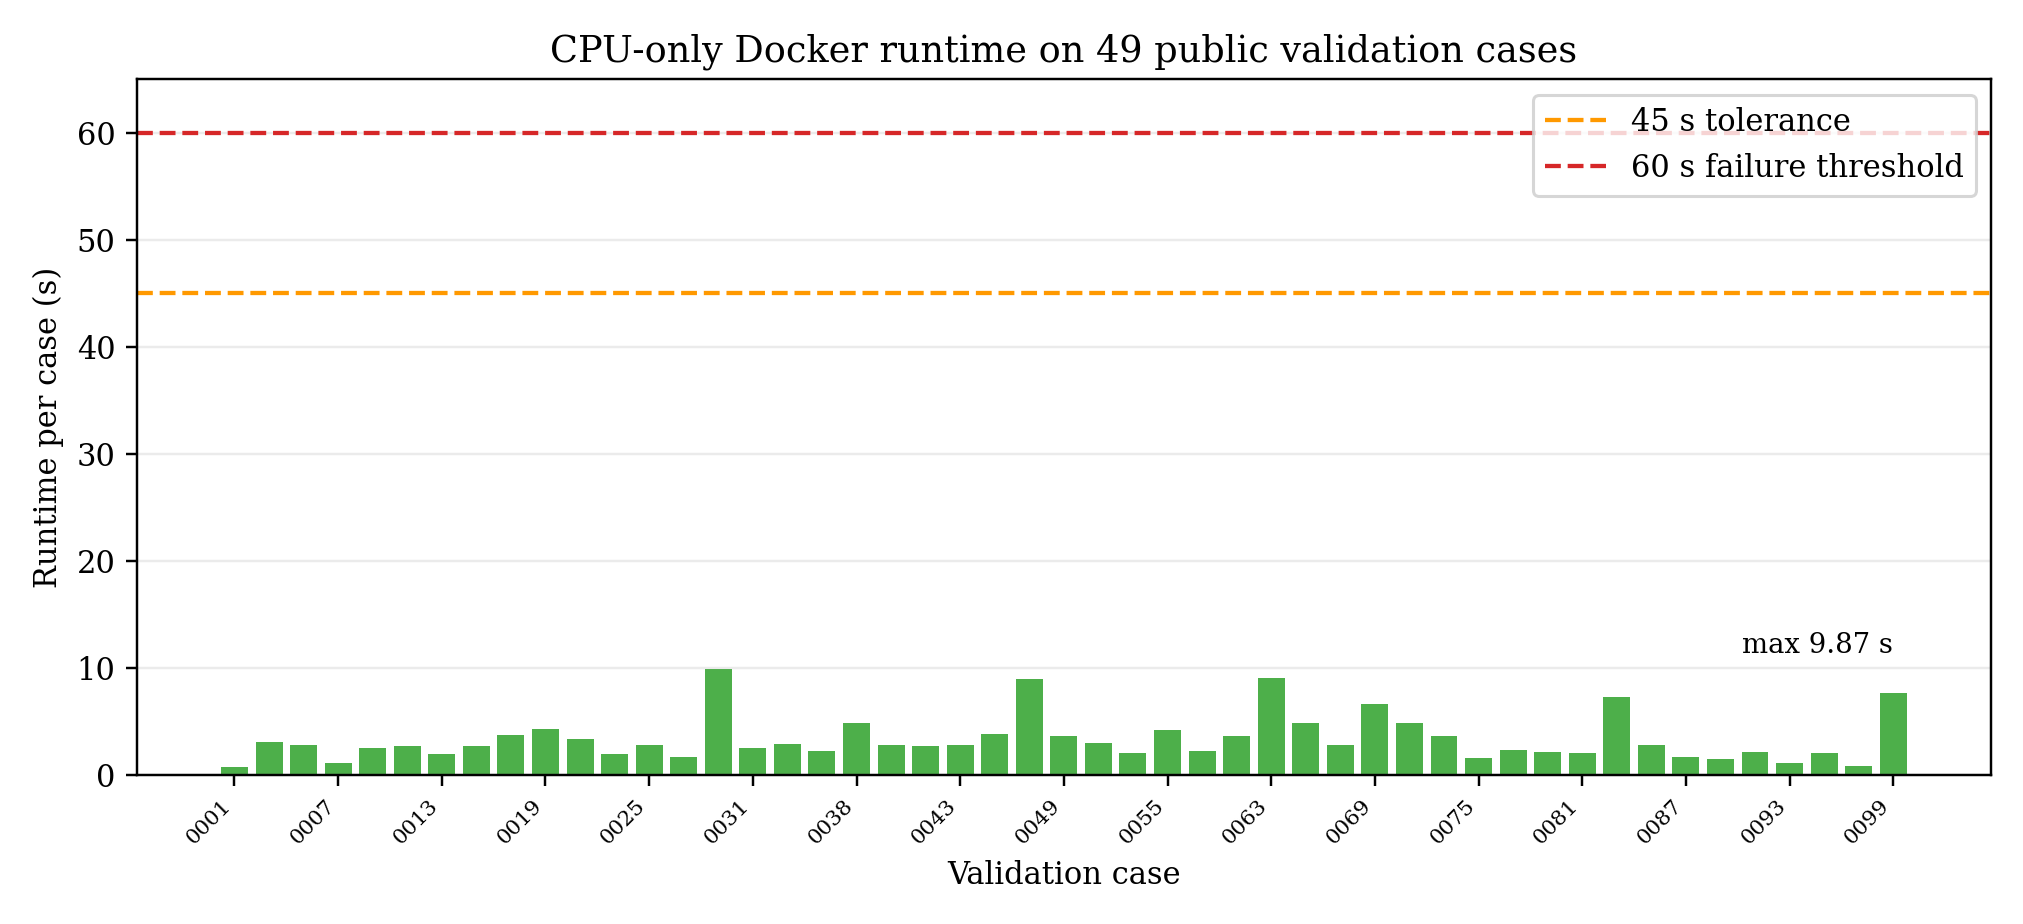
\includegraphics[width=\textwidth]{imgs/medai_runtime.png}
\caption{CPU-only runtime on the public validation set. Dashed lines mark the 45 s tolerance and 60 s failure threshold. No case exceeded either threshold.}
\label{fig:runtime}
\end{figure}

\subsection{Limitations and future work}
\label{sec:limitations}

The method remains dependent on the quality and location of the RECIST marker. If the marker is incomplete, mislabeled, or lies far from the true lesion center, the ROI and component-selection logic may bias the final mask. The deterministic seed-union rule can also slightly enlarge the lesion around the RECIST line, which is usually helpful but may be suboptimal for very thin or ambiguous lesions. Another limitation is that unlabeled and partially labeled scans were not exploited; semi-supervised learning could improve generalization if implemented carefully. Finally, we did not modify the network to accept RECIST as a second image channel, because this would require a more invasive retraining and validation process.

Future work will investigate prompt-aware image encoders, uncertainty-based pseudo labels, stronger lesion-size-aware augmentations, and adaptive post-processing rules that account for the physical RECIST diameter and anisotropic slice spacing without over-constraining irregular lesions.

\section{Conclusion}
\label{sec:conclusion}

We presented a lightweight RECIST-to-3D lesion segmentation method for CPU-only inference. The final approach combines a fine-tuned Lite ENSAM checkpoint with RECIST-aware ROI inference, seed-union post-processing, local connected-component filtering, and hole filling. The central observation is that the RECIST marker can serve as a lesion-specific geometric prior: it identifies where the target component should be, supplies reliable foreground seed voxels, and enables efficient local post-processing. On 49 public validation cases, the submitted method improved over the same-machine Lite ENSAM rerun by 0.0623 DSC and 0.0855 NSD, corresponding to relative gains of 8.9\% and 11.4\%. The method kept the mean CPU runtime at 3.29 s and the maximum official-like runtime below 9 s. These results indicate that RECIST-anchored geometry can improve prompt-to-3D lesion segmentation accuracy without increasing model size or violating CPU-only deployment constraints.

\subsubsection{Acknowledgements}
The authors thank the challenge organizers and data contributors for providing the Pan-cancer Segmentation benchmark. We used the public Lite ENSAM implementation and checkpoint as initialization and integrated it through supervised fine-tuning, checkpoint selection, and task-specific inference-time post-processing. No private external dataset, private pretrained model, pseudo label from previous FLARE winning algorithms, or algorithm distillation was used.

\section*{Disclosure of Interests}
The authors declare no competing interests.

\bibliographystyle{splncs04}
\bibliography{paper}

\newpage
\begin{table}[!htbp]
\caption{Checklist table.}
\centering
\begin{tabular}{ll}
\hline
Requirements & Answer \\
\hline
A meaningful title & Yes \\
\hline
The number of authors ($\leq$6) & 2 \\
\hline
Author affiliations and ORCID & Yes \\
\hline
Corresponding author email is presented & Yes \\
\hline
Validation scores are presented in the abstract & Yes \\
\hline
\begin{tabular}[c]{@{}l@{}}Introduction includes background, related work,\\ and motivation\end{tabular} & Sec.~\ref{sec:intro} \\
\hline
A pipeline/network figure is provided & Fig.~\ref{fig:pipeline} \\
\hline
Pre-processing & Sec.~\ref{sec:preprocessing} \\
\hline
Strategies to use the partial label & Secs.~\ref{sec:preprocessing}, \ref{sec:postprocessing} \\
\hline
Strategies to use the unlabeled images & Not used in the final method \\
\hline
Strategies to improve model inference & Secs.~\ref{sec:postprocessing}, \ref{sec:efficiency} \\
\hline
Post-processing & Sec.~\ref{sec:postprocessing} \\
\hline
Dataset and evaluation metric section & Sec.~\ref{sec:dataset} \\
\hline
Environment setting table & Table~\ref{table:env} \\
\hline
Training protocol table & Table~\ref{table:training} \\
\hline
Ablation study & Sec.~\ref{sec:ablation} \\
\hline
Efficiency evaluation results & Table~\ref{tab:efficiency}, Fig.~\ref{fig:runtime} \\
\hline
Visualized segmentation examples & Fig.~\ref{fig:qualitative} \\
\hline
Limitation and future work are presented & Sec.~\ref{sec:limitations} \\
\hline
Reference format is consistent & Yes \\
\hline
\end{tabular}
\end{table}

\end{document}
